% !TEX root = ../ApproxDA-TransUNet.tex
\section{Method}
\label{sec:method}

\subsection{Architecture overview}

ApproxDA-TransUNet keeps the hybrid CNN--ViT encoder and decoder of DA-TransUNet~\cite{sun2024datransunet}, with an R50-ViT-B/16 backbone (Fig.~\ref{fig:framework}). Three CNN stages produce features at strides 2, 4, and 8, and a 12-layer ViT processes $14{\times}14$ patch tokens. ApproxDABlocks are placed at the bottleneck and at the three skip connections (512 channels at $28^2$, 256 at $56^2$, 64 at $112^2$). The public DA-TransUNet implementation applies dual attention only at the bottleneck and the 512- and 256-channel skips, because its decoder selects the block by the decoder channel count rather than the skip channel count; we keep that implementation unchanged as the baseline and additionally place a block at the 64-channel skip.

Each ApproxDABlock keeps the layout of the DA-TransUNet block and replaces only its attention modules (Fig.~\ref{fig:block}). Each branch first reduces the $C$ input channels to $C/16$ with a $3{\times}3$ convolution, batch normalization, and ReLU, as in DA-TransUNet; the PAM and CAM branches then apply the approximated attention described below, followed by another $3{\times}3$ convolution block. The two branches are fused and projected back to $C$ channels.

\begin{figure*}[t]
  \centering
  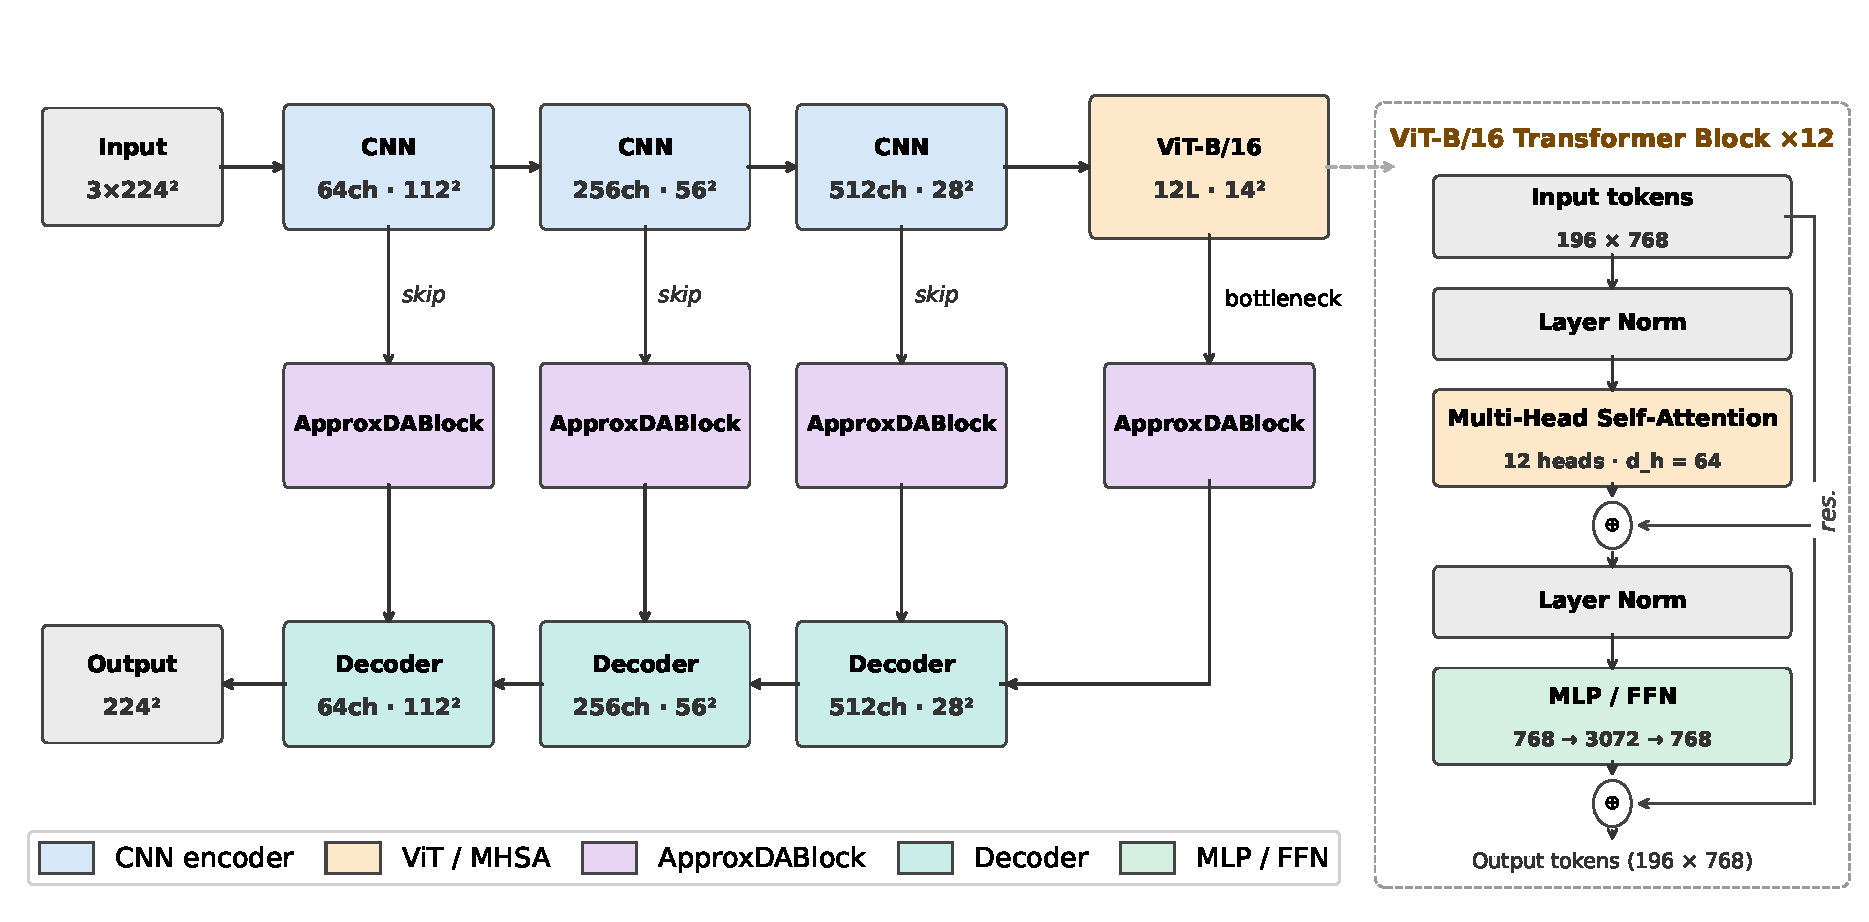
\includegraphics[width=0.92\textwidth]{figures/approxda_overview}
  \caption{ApproxDA-TransUNet. ApproxDABlocks (windowed low-rank PAM + grouped CAM + routing) are placed at all three skip connections and at the bottleneck; the CNN--ViT backbone of DA-TransUNet is unchanged.}
  \label{fig:framework}
\end{figure*}

\begin{figure*}[t]
  \centering
  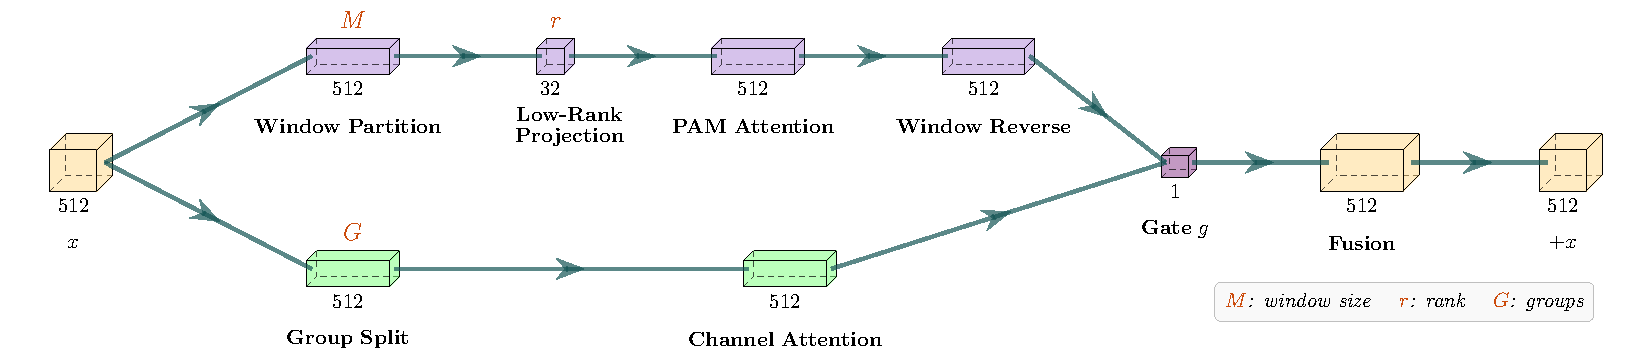
\includegraphics[width=0.92\textwidth]{figures/approxda_block}
  \caption{ApproxDABlock with three independently controllable approximation axes: spatial scope ($M$), affinity resolution ($r$), and channel interaction ($G$). Each branch reduces the input to $C/16$ channels before attention, as in DA-TransUNet; the branch outputs are fused by the per-channel routing vector $\mathbf{g}$ and projected back to $C$ channels by a $1{\times}1$ convolution.}
  \label{fig:block}
\end{figure*}
% TODO(figure): the gate cube in approxda_block.pdf is labelled "1" (scalar);
% relabel to C (per-channel vector) to match Eq. (5). Source file not in repo.

\textbf{Approximation axes.} The original dual-attention block computes dense spatial and channel attention over the full feature map. ApproxDA-TransUNet approximates it along three independent axes. \emph{Spatial scope} (window size $M$) controls how far PAM reaches; $M{\times}M$ windows trade long-range context for lower cost. \emph{Affinity resolution} (rank $r$) controls how finely attention is computed inside a window; higher $r$ approaches exact attention. \emph{Channel interaction} (groups $G$) restricts CAM to interactions within $G$ channel groups. Any two of $\{M, r, G\}$ can be held fixed while the third varies.

\subsection{Spatial approximation}

\textbf{Full PAM.} Following~\cite{fu2019dual}, let $\mathbf{A} \in \mathbb{R}^{C \times N}$ be the (channel-reduced) input of the attention module, $N = HW$, and let $\mathbf{B}, \mathbf{C} \in \mathbb{R}^{C' \times N}$ and $\mathbf{D} \in \mathbb{R}^{C \times N}$ be query, key, and value features produced by $1{\times}1$ convolutions, with columns $\mathbf{B}_j$, $\mathbf{C}_i$, $\mathbf{D}_i$ and $C' = \max(1, C/8)$ as in the DA-TransUNet implementation. PAM computes
\begin{equation}
  s_{ji} = \frac{\exp(\mathbf{B}_j^{\top}\mathbf{C}_i)}{\sum_{i'=1}^{N}\exp(\mathbf{B}_j^{\top}\mathbf{C}_{i'})}, \quad
  \mathbf{E}_j = \alpha \sum_{i=1}^{N} s_{ji}\,\mathbf{D}_i + \mathbf{A}_j,
  \label{eq:pam_full}
\end{equation}
where $\alpha$ is a learned scalar initialized to 0. The $N{\times}N$ attention matrix costs $\mathcal{O}(N^2C)$.

\textbf{Window partitioning.} Following~\cite{liu2021swin}, the map is split into non-overlapping $M{\times}M$ windows with $M \leftarrow \min(M,H,W)$, and Eq.~\eqref{eq:pam_full} is evaluated inside each window over its $N_w = M^2$ positions. This reduces the cost to $\mathcal{O}(NM^2C)$; the window outputs are then merged back to the $H{\times}W$ grid.

\textbf{Low-rank projection.} Following~\cite{wang2020linformer}, keys and values inside each window, $\mathbf{C} \in \mathbb{R}^{C' \times N_w}$ and $\mathbf{D} \in \mathbb{R}^{C \times N_w}$, are compressed along the token axis by a learned projection $\mathbf{P} \in \mathbb{R}^{N_w \times r}$ shared across windows:
\begin{equation}
  \tilde{\mathbf{C}} = \mathbf{C}\mathbf{P} \in \mathbb{R}^{C' \times r}, \qquad \tilde{\mathbf{D}} = \mathbf{D}\mathbf{P} \in \mathbb{R}^{C \times r}.
  \label{eq:lowrank}
\end{equation}
Each query then attends to the $r$ projected keys instead of the $N_w$ original ones:
\begin{equation}
  \tilde{s}_{jk} = \frac{\exp(\mathbf{B}_j^{\top}\tilde{\mathbf{C}}_k)}{\sum_{k'=1}^{r}\exp(\mathbf{B}_j^{\top}\tilde{\mathbf{C}}_{k'})}, \quad
  \mathbf{E}_j = \alpha \sum_{k=1}^{r} \tilde{s}_{jk}\,\tilde{\mathbf{D}}_k + \mathbf{A}_j,
  \label{eq:pam_lr}
\end{equation}
so the per-window attention matrix is $N_w{\times}r$ instead of $N_w{\times}N_w$, and the total cost becomes $\mathcal{O}(NrC)$. As in~\cite{fu2019dual}, no temperature scaling is applied. When $M$ is clamped to a smaller map, the first $N_w$ rows of $\mathbf{P}$ are used. Hence $M{=}112$ gives a single window per map (global spatial scope), but the attention remains rank-$r$ and is \emph{not} exact full PAM; omitting the projection ($\tilde{\mathbf{C}}{=}\mathbf{C}$, $\tilde{\mathbf{D}}{=}\mathbf{D}$) recovers exact attention within each window.

\subsection{Channel approximation}

CAM~\cite{fu2019dual} computes a $C{\times}C$ channel affinity at $\mathcal{O}(C^2N)$ cost. We split the $C$ channels into $G$ groups of $C_g = C/G$ channels and compute attention within each group. For group $g$ with channel rows $\mathbf{A}^{(g)}_1,\dots,\mathbf{A}^{(g)}_{C_g} \in \mathbb{R}^{N}$,
\begin{equation}
\begin{aligned}
  x^{(g)}_{ij} &= \frac{\exp(-\mathbf{A}^{(g)}_i \cdot \mathbf{A}^{(g)}_j)}{\sum_{k=1}^{C_g}\exp(-\mathbf{A}^{(g)}_i \cdot \mathbf{A}^{(g)}_k)}, \\
  \mathbf{E}^{(g)}_i &= \beta \sum_{j=1}^{C_g} x^{(g)}_{ij}\,\mathbf{A}^{(g)}_j + \mathbf{A}^{(g)}_i,
\end{aligned}
  \label{eq:groupedcam}
\end{equation}
where $\beta$ is a learned scalar initialized to 0. Following the official DANet and DA-TransUNet implementations, the channel affinity is negated before the softmax (implemented as $\max_k \mathbf{A}_i\cdot\mathbf{A}_k - \mathbf{A}_i\cdot\mathbf{A}_j$, which is equivalent under the softmax). Grouping reduces the cost to $\mathcal{O}(C^2N/G)$, and $G{=}1$ recovers the CAM module of DA-TransUNet exactly. When a reduced map has fewer than $G$ channels (4 channels at the 64-channel skip), one channel per group is used.

\subsection{Routing and complexity}

Let $\mathbf{X}$ be the block input with $C$ channels, and let $\phi$ denote a $3{\times}3$ convolution with batch normalization and ReLU. The block output is
\begin{equation}
\begin{aligned}
  \mathbf{P} &= \phi_{51}\big(\mathrm{PAM}(\phi_{5a}(\mathbf{X}))\big), \quad
  \mathbf{Q} = \phi_{52}\big(\mathrm{CAM}(\phi_{5c}(\mathbf{X}))\big), \\
  \mathbf{Y} &= \mathrm{ReLU}\big(\mathbf{W}_f\,(\mathbf{g} \odot \mathbf{P} + (\mathbf{1}-\mathbf{g}) \odot \mathbf{Q})\big),
\end{aligned}
  \label{eq:fusion}
\end{equation}
where $\phi_{5a}, \phi_{5c}$ map $C \to C/16$ channels, $\mathbf{W}_f$ is a $1{\times}1$ convolution back to $C$ channels (with dropout during training), and $\mathbf{g} \in [0,1]^{C/16}$ is a per-channel routing vector broadcast over positions, set by the routing mode:
\begin{center}
\small
\begin{tabular}{@{}ll@{}}
  PAM-only: & $\mathbf{g} = \mathbf{1}$ \\
  CAM-only: & $\mathbf{g} = \mathbf{0}$ \\
  fixed:    & $\mathbf{g} = 0.5\cdot\mathbf{1}$ \\
  learned:  & $\mathbf{g} = \sigma(\mathbf{W}_g\,\mathrm{GAP}(\mathbf{X}))$ \\
\end{tabular}
\end{center}
PAM-only and CAM-only routing build only the branch they use. With exact attention ($M$ covering the whole map, no projection), $G{=}1$, and $\mathbf{g}{=}0.5\cdot\mathbf{1}$, the block reduces to the DA-TransUNet block up to a rescaling of $\mathbf{W}_f$.
The network is trained with $\mathcal{L} = \tfrac{1}{2}\mathcal{L}_{\mathrm{Dice}} + \tfrac{1}{2}\mathcal{L}_{\mathrm{CE}}$, as in DA-TransUNet.

Windowing and low-rank projection reduce the PAM attention matrix from $N{\times}N$ to $N{\times}r$, a factor of $N/r \approx 390$ at the $112^2$ skip with $r{=}32$. End-to-end cost is dominated by the unchanged backbone: the ViT encoder alone holds 85.1M of the parameters and 17.4 of the GFLOPs (fvcore, one $224{\times}224$ slice), and the CNN encoder and decoder most of the rest. The attention blocks of DA-TransUNet account for 0.87 GFLOPs; those of ApproxDA-TransUNet (PAM-only, $M{=}28$, $r{=}32$) for 0.40 GFLOPs, compared with 1.37 GFLOPs for the same blocks with exact attention. The full networks have 107.95M parameters / 30.20 GFLOPs (DA-TransUNet) and 105.99M / 29.73 GFLOPs (ApproxDA-TransUNet); we therefore do not claim substantial whole-network acceleration.
\todo{optional: block-level latency / memory on the same GPU.}
